\documentclass[12pt,a4paper,openright]{report}
\usepackage[italian]{babel}
\usepackage[utf8]{inputenc}
\usepackage{hyperref}
\usepackage{url}
%\usepackage{natbib}
\usepackage{graphicx}
\usepackage{makeidx}
\usepackage{listings}
\usepackage[square,numbers,sort]{natbib}
\usepackage{tabularx}
\usepackage{float}

% version
\newcommand{\versionmajor}{0}
\newcommand{\versionminor}{1}
\newcommand{\versionpatch}{2}
\newcommand{\version}{\versionmajor.\versionminor.\versionpatch}
\typeout{Document version: \version}

\title{\LARGE
    Ontologie nel dominio energetico applicate alla gestione di un Prosumer \\ \small Secondo e terzo assignment per il corso di Web Semantico
}

\author{
    Eddie Barzi \\ \small eddie.barzi@studio.unibo.it
    \and
    Angela Cortecchia \\ \small angela.cortecchia@studio.unibo.it
}

\date{\small Anno Accademico 2022-2023}
\makeindex

\begin{document}
\maketitle

\tableofcontents

\chapter{Introduzione}
\chapter{Analisi del dominio e del contesto}
In questa sezione viene riportata la modellazione di classi e proprietà che compongono l'ontologia.


\section{Analisi del dominio}
Il dominio è inerente all'energia, in maniera specifica al Prosumer, ovvero un'entità che può sia produrre che consumare energia.
Un Prosumer è caratterizzato da:

\begin{itemize}
    \item Un profilo di carico equivalente o consumo;
    \item Un sistema di generazione;
    \item Un sistema di accumulo dell'energia o storage;
    \item Due o più contatori, detti anche punti di misura.
\end{itemize}

Un sistema di accumulo può essere monodirezionale, ovvero può assorbire energia elettrica solo dall’impianto di produzione, oppure bidirezionale, cioè può assorbire energia elettrica sia dall’impianto di produzione che dalla rete con obbligo di connessione di terzi.
Il principale elemento differenziante è quindi se lo storage assorbe energia esclusivamente dall’impianto di produzione.

In base alla configurazione (descritta in seguito), l'impianto può avere due o tre contatori:
\begin{itemize}
    \item Contatore M1: è il contatore di scambio con la rete di distribuzione, e misura l’energia scambiata (assorbita o immessa) con la rete.
    \item Contatore M2: è il contatore che misura l’energia scambiata nel punto di produzione (ovvero la combinazione dell’energia prodotta dal generatore con l’energia fornita o assorbita dal sistema di accumulo).
    \item Contatore M3: quando presente (configurazione 3 descritta più avanti), serve a misurare l’energia di carico e scarico del sistema di accumulo (tipicamente, una batteria elettrica).
\end{itemize}

È noto che il prosumer possa avere tre tipi di configurazioni, ovvero:
\begin{itemize}
    \item Configurazione 1:
          \begin{itemize}
              \item Sistema di accumulo monodirezionale, situato lato produzione e caratterizzato da corrente continua;
              \item Presenza dei contatori M1 e M2, assenza del contatore M3.
          \end{itemize}
    \item Configurazione 2:
          \begin{itemize}
              \item Sistema di accumulo bidirezionale, situazio lato produzione e caratterizzato da corrente che può essere sia alternata che continua;
              \item Presenza dei contatori M1, M2, assenza del contatore M3.
          \end{itemize}
    \item Configurazione 3:
          \begin{itemize}
              \item Sistema di accumulo bidirezionale, situato lato post-produzione e caratterizzato da corrente alternata;
              \item Presenza dei contatori M1, M2 e M3.
          \end{itemize}
\end{itemize}

\section{Classi}
L'ontologia è stata sviluppata focalizzandosi sul ruolo del prosumer e delle sue caratteristiche.
Di conseguenza è stato pensato di modellare come classi principali:
\begin{itemize}
    \item \textbf{Prosumer};
    \item Profilo di consumo, chiamato \textbf{Load};
    \item Sistema di generazione, chiamato \textbf{Generator};
    \item Sistema di accumulo, chiamato \textbf{Storage System}, composto da uno o più \textbf{Energy Storage} o \textbf{Battery};
    \item Contatore, chiamato \textbf{Energy Meter}.
\end{itemize}

\section{Proprietà}

\section{Data Properties}
\chapter{Modellazione e sviluppo dell'ontologia}
Durante tutto lo sviluppo dell'ontologia si è cercato il più possibile di utilizzare ontologie già esistenti, in modo da non dover ripetere la modellazione di classi e proprietà già definite e rendere tutto più consistente.

\section{Ontologie importate}

In particolare, le ontologie prese in considerazione sono:
\begin{itemize}
    \item \texttt{Battery}\cite{battery_kyrillos}: ontologia sviluppata da Kyrillos Ntronov per la modellazione di uno Storage System;
    \item \texttt{SAREF}\cite{saref}: ontologia sviluppata dall'ETSI (European Telecommunications Standards Institute) con l'obiettivo di fornire un riferimento standard per la rappresentazione semantica delle apparecchiature intelligenti (smart appliances) e dei loro dati;
    \item \texttt{InterConnect}\cite{interconnect}: insieme di ontologie per supportare la modellazione e l'integrazione semantica di dati e informazioni nel settore dell'energia e dell'elettricità. In particolare è stata utilizzata l'ontologia \textit{ic-data}\cite{ic-data} per la modellazione di misurazioni e sequenze di misurazioni;
\end{itemize}

Considerando lo scopo didattico del progetto e il fallimento nell'importazione automatica di alcune ontologie su Protègè, si è proceduto a semplificare alcune classi importate manualmente da altre ontologie. Ad esempio, sono state rimosse alcune restrizioni non strettamente necessarie nelle classi TimeSeries e DataPoint dell'ontologia ic-data.

\section{Prosumer}
Il prosumer è l'entità principale dell'ontologia, ciò che andrà a contenere le entità caratterizzanti.

\begin{figure}[!ht]
    \centering
    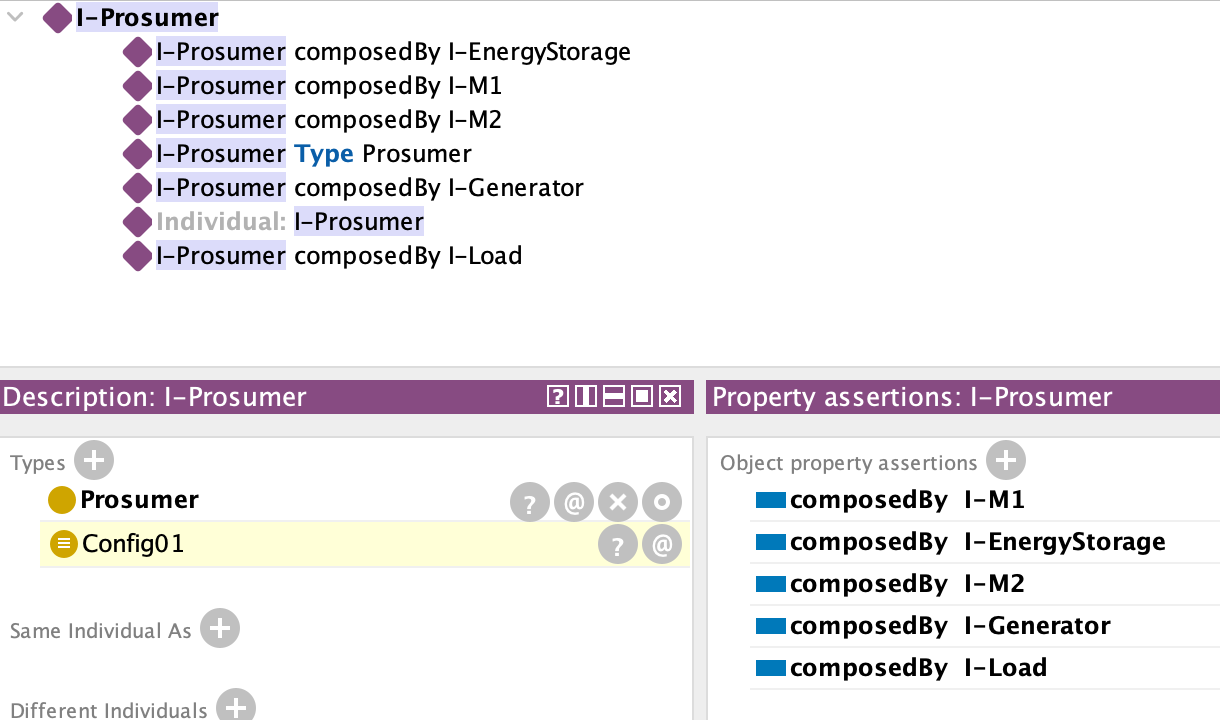
\includegraphics[width=12cm]{images/individual_prosumer.png}
    \caption{Prosumer applicato a un individuo su Protègè.}
    \label{fig:individual_prosumer}
\end{figure}

Come si può notare nell'immagine \ref*{fig:individual_prosumer}, al prosumer vengono assegnati altri individui tramite le proprietà, grazie a ciò il reasoner è in grado di inferire la tipologia di configurazione.
In questo caso è di tipo Config01, siccome Energy Storage rispetta le caratteristiche della configurazione, come verrà mostrato nelle sezioni successive.

\subsection{Configuration}
Per stabilire la tipologia di configurazione, è stata creata la sottoclasse Configuration che a sua volta possiede le sottoclassi Config01, Config02 e Config03.

\begin{figure}[!ht]
    \centering
    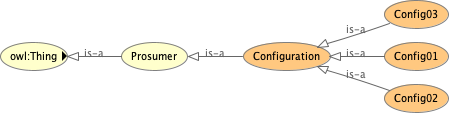
\includegraphics[width=12cm]{images/pros_graph.png}
    \caption{Grafico creato su Protègè tramite il plugin OWLViz.}
    \label{fig:pros_graph}
\end{figure}

Per specificare le caratteristiche di ogni configurazione, sono state espresse le condizioni necessarie e sufficienti. Per ogni configurazione sono presenti:
\begin{verbatim}
    Prosumer 
     and (composedBy some Generator) 
     and (composedBy some Load) 
     and (composedBy some M1) 
     and (composedBy some M2) 
\end{verbatim}

Mentre, in aggiunta per ogni configurazione:
\begin{itemize}
    \item Configurazione 01: condizioni necessarie e sufficienti: \begin{verbatim}
        and (composedBy some 
            (StorageSystem 
             and (hasDirection some Monodirectional) 
             and (hasLocation some Production) 
             and (hasPowerType some DC)))
    \end{verbatim}
          condizioni necessarie: \begin{verbatim}
        Prosumer and (not (composedBy some M3))
    \end{verbatim}
    \item Configurazione 02: condizioni necessarie e sufficienti: \begin{verbatim}
        and (composedBy some 
            (StorageSystem 
             and (hasDirection some Bidirectional) 
             and (hasLocation some Production) 
             and (hasPowerType some (AC or DC))))
    \end{verbatim}
          condizioni necessarie: \begin{verbatim}
        Prosumer and (not (composedBy some M3))
    \end{verbatim}
    \item Configurazione 03: condizioni necessarie e sufficienti \begin{verbatim}
         and (composedBy some M3) 
         and (composedBy some 
            (StorageSystem 
             and (hasDirection some Bidirectional) 
             and (hasLocation some Post-Production)
             and (hasPowerType some AC)))
    \end{verbatim}
\end{itemize}


\section{Generator}
IL generatore rappresenta l'entità che produce energia ed è presente in tutti i prosumer.
L'energia prodotta dal generatore servirà a soddisfare il Load, a caricare lo Storage System e quella in eccesso verrà immessa nella rete.
\begin{figure}[H]
    \centering
    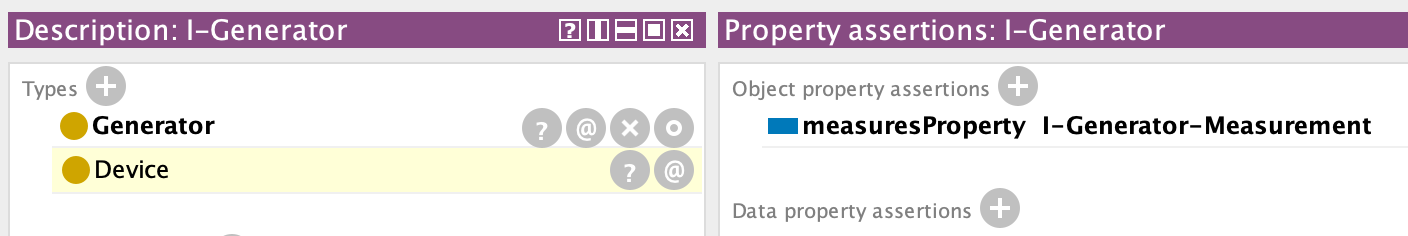
\includegraphics[width=12cm]{images/individual_generator.png}
    \caption{Istanza di un individuo di tipo generatore.}
    \label{fig:individual_generator}
\end{figure}

Per monitorare l'energia prodotta dal generatore, è stata definita un'istanza della classe "Time Series" (figura \ref{fig:individual_genmeas}), importata dall'ontologia ic-data. In questo modo si può definire un intervallo temporale e creare una sequenza di "Data Point"(anch'essa classe importata da ic-data), uno per ogni intervallo di tempo.
\begin{figure}[H]
    \centering
    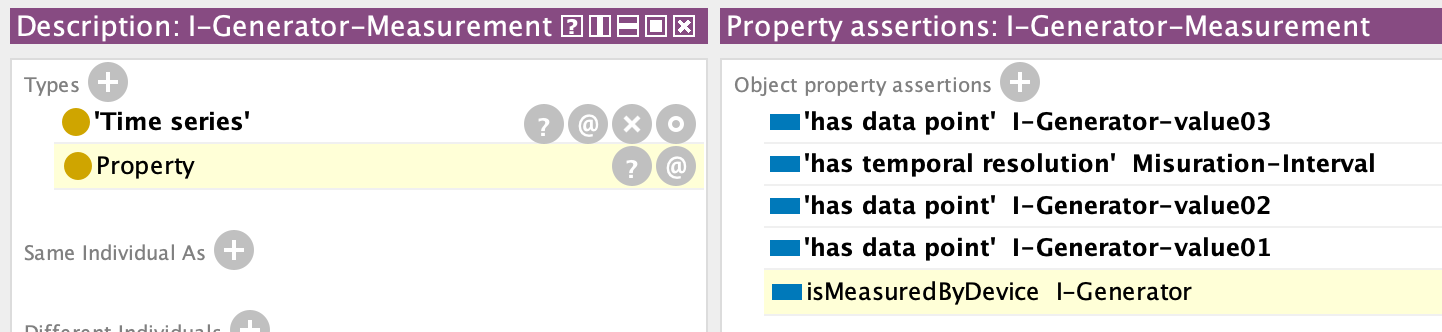
\includegraphics[width=12cm]{images/individual_genmeas.png}
    \caption{Istanza di un individuo di tipo Time Series per il generatore.}
    \label{fig:individual_genmeas}
\end{figure}
Ogni singolo "GeneratorMeasurement" è quindi sottoclasse di Data Point e rappresenta un'osservazione dell'energia prodotta dal generatore in un intervallo di tempo specificato dal timestamp (figura \ref{fig:individual_genval3}).
\begin{figure}[H]
    \centering
    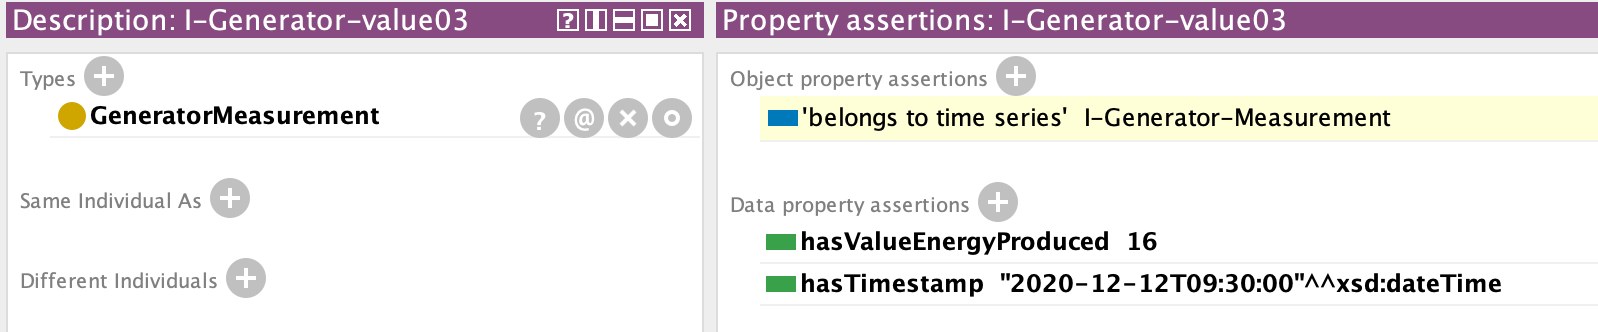
\includegraphics[width=12cm]{images/individual_genval3.png}
    \caption{Istanza di un individuo di tipo GeneratorMeasurement.}
    \label{fig:individual_genval3}
\end{figure}


\section{Load}
Il Load rappresenta il profilo di carico equivalente, anche detto consumo, del prosumer.
\begin{figure}[H]
    \centering
    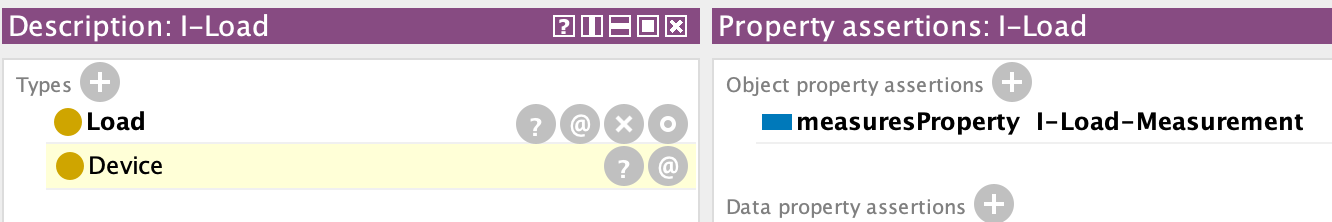
\includegraphics[width=12cm]{images/individual_load.png}
    \caption{Istanza di un individuo di tipo Load.}
    \label{fig:individual_load}
\end{figure}
Analogamente per quanto fatto per il generatore, anche per il Load è stata definita un'istanza della classe "Time Series" (figura \ref{fig:individual_loadmes}) e ogni singolo "LoadMeasurement"
è sottoclasse di Data Point (figura \ref{fig:individual_loadval3}).
\begin{figure}[H]
    \centering
    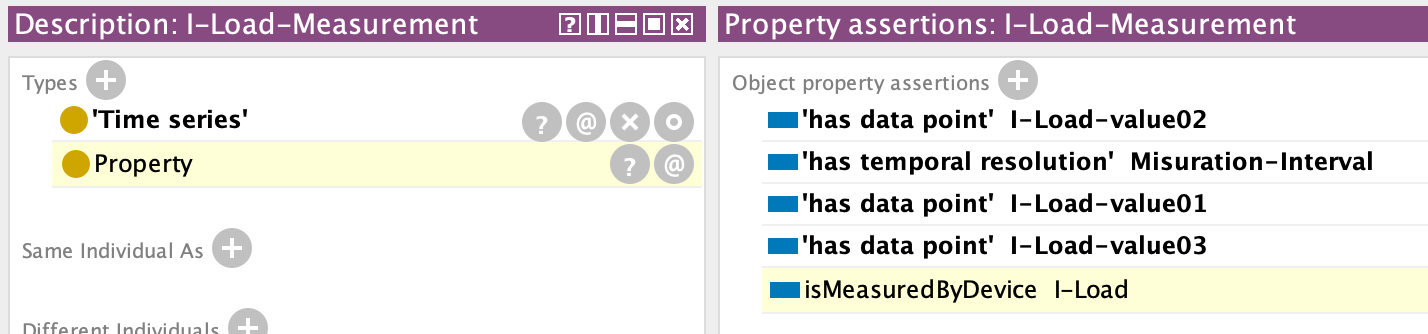
\includegraphics[width=12cm]{images/individual_loadmes.png}
    \caption{Istanza di un individuo di tipo Time Series per il Load.}
    \label{fig:individual_loadmes}
\end{figure}
In questo modo si va a specificare l'energia consumata dal prosumer in un intervallo di tempo specificato dal timestamp, fornendo una visione dettagliata dell'utilizzo dell'energia da parte del prosumer nel corso del tempo.
\begin{figure}[H]
    \centering
    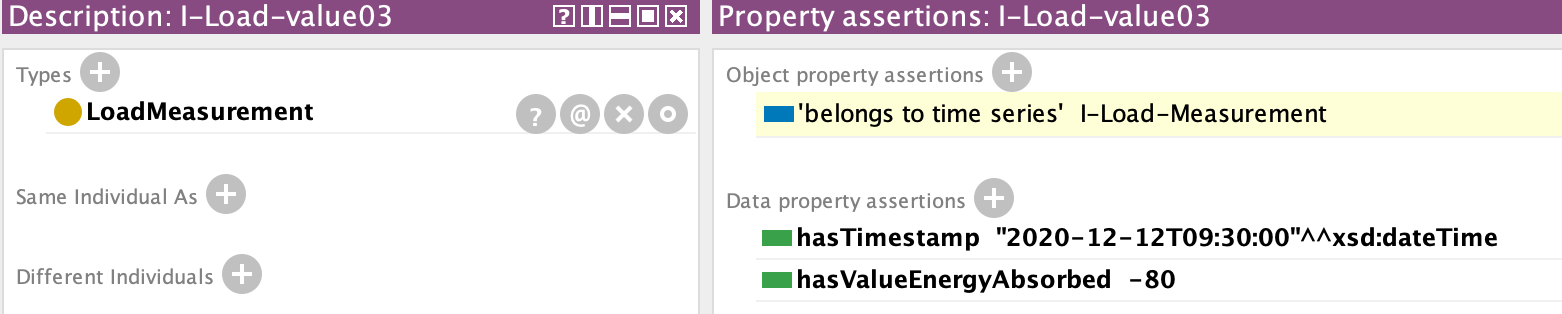
\includegraphics[width=12cm]{images/individual_loadval3.png}
    \caption{Istanza di un individuo di tipo LoadMeasurement.}
    \label{fig:individual_loadval3}
\end{figure}

\section{Storage System}
Lo Storage System è l'entità che rappresenta il sistema di accumulo dell'energia di un prosumer. Viene utilizzato per immagazzinare l'energia ed eventualmente per fornirla al prosumer in caso di necessità.
In questo caso è stata estesa l'ontologia \textit{Battery} sviluppata da Kyrillos, aggiungendo informazioni quali il tipo di corrente (AC o DC), la direzione del flusso energetico (monodirezionale o bidirezionale) e il posizionamento (produzione o post-produzione), utili per identificare la configurazione del prosumer.
In figura \ref{fig:individual_storagesystem} viene mostrata l'istanza di una classe StorageSystem, composto da due batterie, il tipo di corrente, la direzione del flusso e il posizionamento.
\begin{figure}[H]
    \centering
    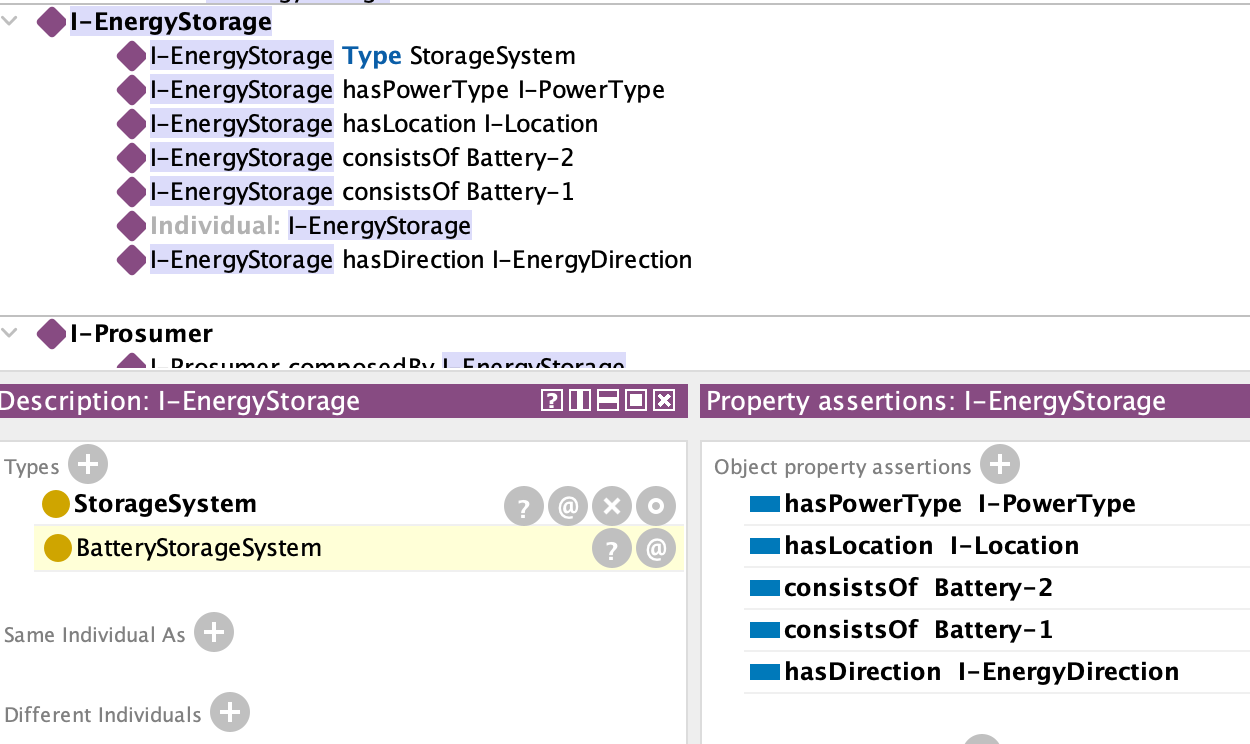
\includegraphics[width=12cm]{images/individual_storagesystem.png}
    \caption{Istanza di un individuo di tipo StorageSystem.}
    \label{fig:individual_storagesystem}
\end{figure}
Nella figura \ref{fig:individual_bat1} viene mostrata l'istanza di una classe Battery, in questo caso la Batteria 1 facente parte dello Storage System. Questa classe è utile per specificare le caratteristiche della batteria, salvate come Data Property.
\begin{figure}[H]
    \centering
    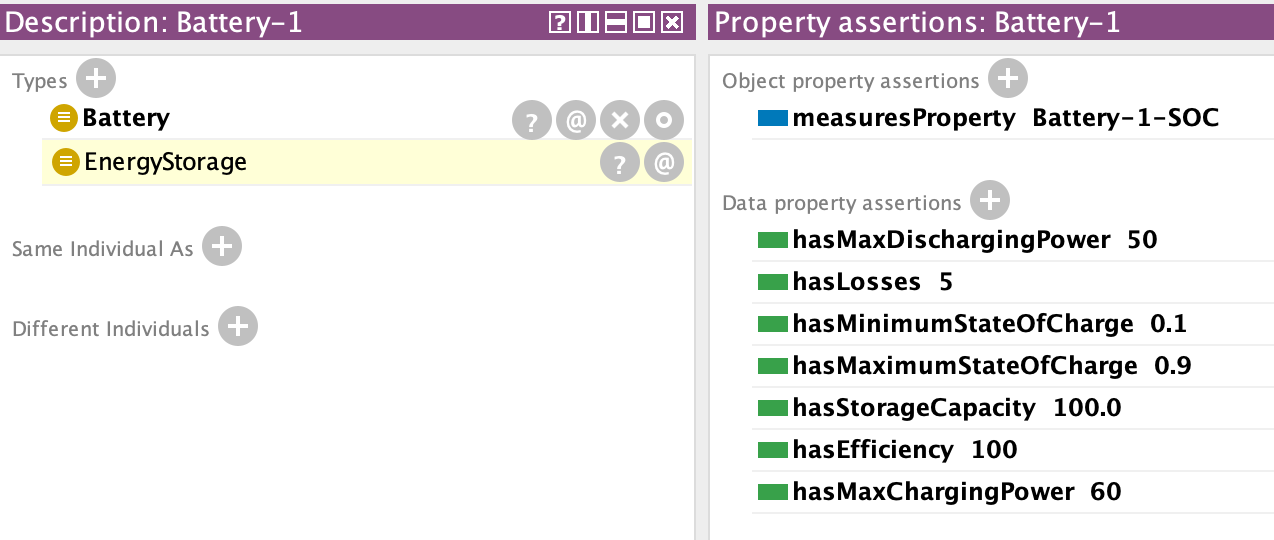
\includegraphics[width=12cm]{images/individual_bat1.png}
    \caption{Istanza di un individuo di tipo Battery.}
    \label{fig:individual_bat1}
\end{figure}
La classe StateOfCharge è sottoclasse di Time Series, quindi la sua utilità è quella di avere il riferimento a una sequenza di misurazioni.
\begin{figure}[H]
    \centering
    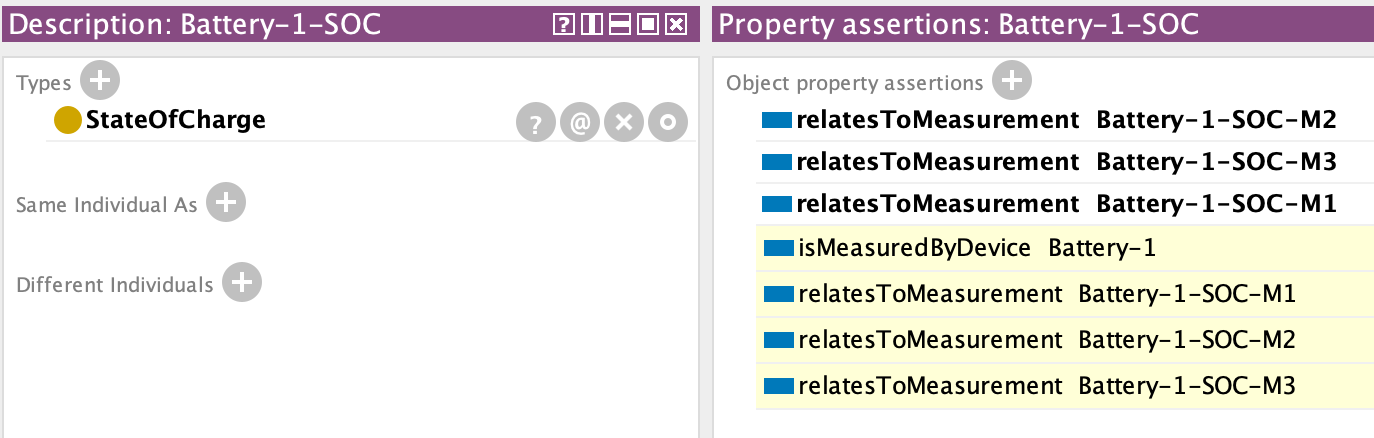
\includegraphics[width=12cm]{images/individual-batterysoc.png}
    \caption{Istanza di un individuo di tipo StateOfCharge.}
    \label{fig:individual-batterysoc}
\end{figure}
Ogni misurazione è rappresentata da un'istanza di StateOfChargeMeasurement, sottoclasse di Data Point.
In figura \ref{fig:individual_batterym3} si possono notare le due Data Property inferite grazie alle regole SWRL descritte nella sezione \ref{sec:swrl}.
\begin{figure}[H]
    \centering
    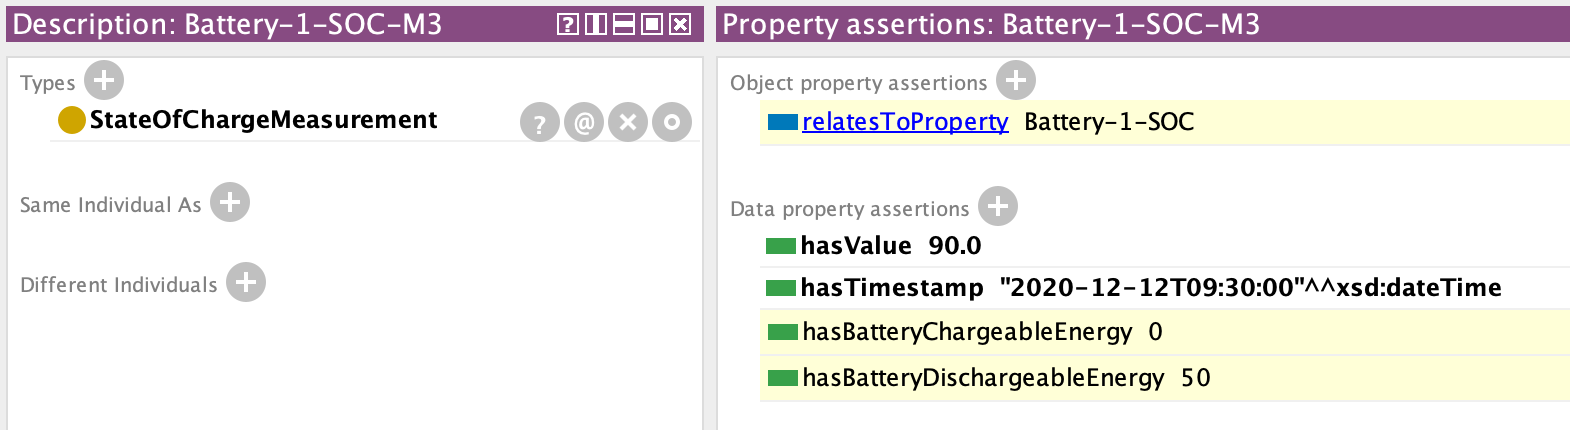
\includegraphics[width=12cm]{images/individual-batterym3.png}
    \caption{Istanza di un individuo di tipo StateOfChargeMeasurement.}
    \label{fig:individual_batterym3}
\end{figure}

\section{Energy Meter}
L'Energy Meter è l'entità che rappresenta il contatore di energia di un prosumer. Come già descritto nella sezione \ref{sec:analisi_dominio} un prosumer deve avere un contatore di tipo M1, un contatore di tipo M2 e, solo per la configurazione tre, un contatore di tipo M3.
Questi tre tipi di contatori sono stati rappresentati con tre classi distinte, definite come sottoclassi della classe EnergyMeter.

In figura \ref{fig:individual_m1} viene mostrata l'istanza di una classe M1, in questo caso il contatore M1 facente parte del prosumer.
\begin{figure}[H]
    \centering
    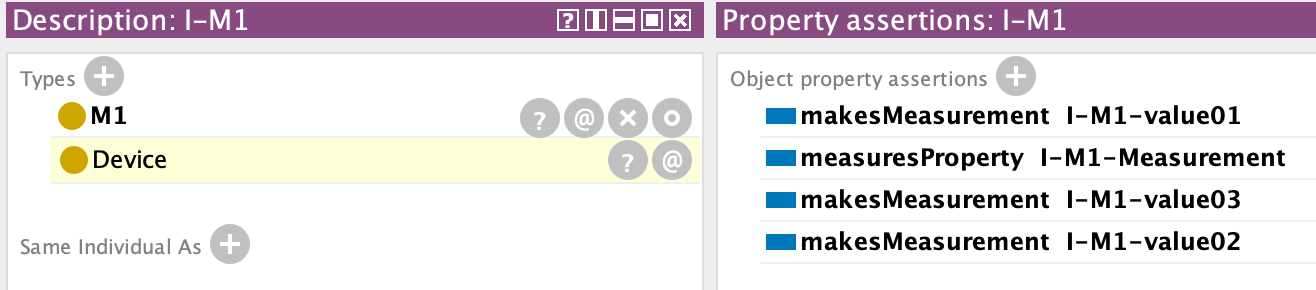
\includegraphics[width=12cm]{images/individual_m1.png}
    \caption{Istanza di un individuo di tipo M1.}
    \label{fig:individual_m1}
\end{figure}

Come per gli altri componenti, anche il contatore ha una sequenza di misurazioni, rappresentata dalla classe Time Series.

\begin{figure}[H]
    \centering
    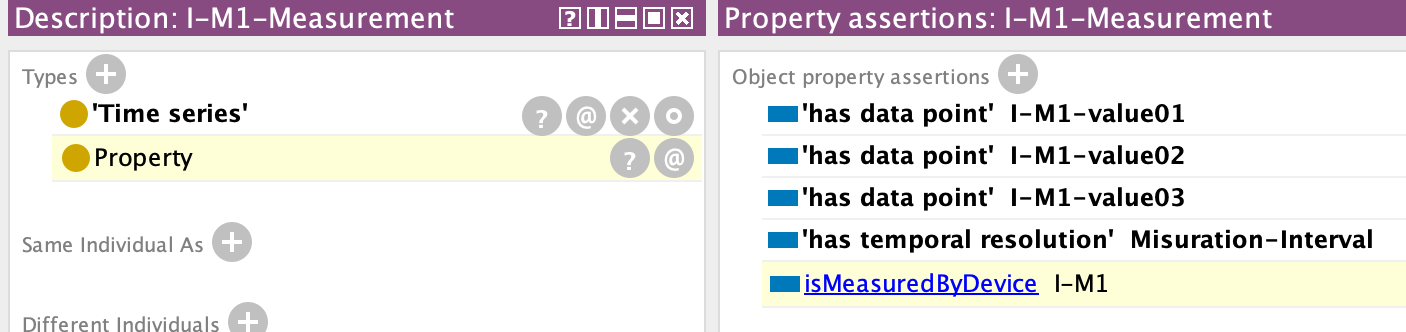
\includegraphics[width=12cm]{images/individual_m1meas.png}
    \caption{Istanza di un individuo di tipo Time Series per M1.}
    \label{fig:individual_m1meas}
\end{figure}

Ogni misurazione è rappresentata da un'istanza di EnergyMeterMeasurement, sottoclasse di Data Point. Si può notare dalla figura \ref{fig:individual_m1val3} che nel caso dei contatori nella misurazione è stato inserito solo il valore del timestamp, in quanto il valore dell'energia scambiata è calcolato con le query SPARQL descritte nella sezione \ref{sec:sparql}.

\begin{figure}[H]
    \centering
    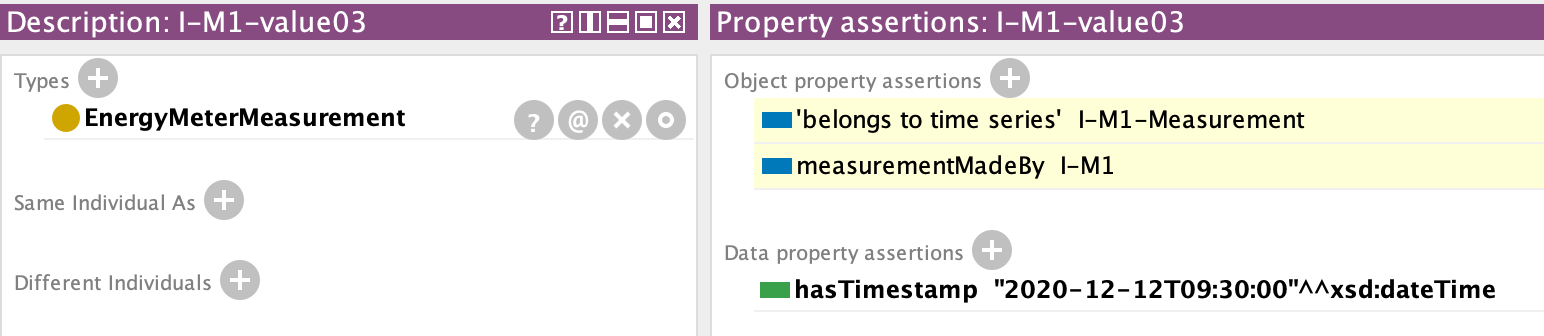
\includegraphics[width=12cm]{images/individual_m1val3.png}
    \caption{Istanza di un individuo di tipo EnergyMeterMeasurement}
    \label{fig:individual_m1val3}
\end{figure}
\chapter{Interrogazione dell'ontologia}

\section{SWRL}\label{sec:swrl}
Sono state utilizzate regole SWRL per consentire al reasoner di inferire ulteriori informazioni sull'ontologia, in particolare riguardo al valore di energia che una batteria può effettivamente assorbire o fornire, in uno specifico intervallo di tempo.

Le regole SWRL implementate permettono di calcolare il valore di queste due Data Property, che saranno utilizzate poi nelle query SPARQL:
\begin{itemize}
    \item \texttt{hasBatteryChargeableEnergy}: effettiva capacità di carica di una batteria, ovvero l'energia che la batteria è in grado di immagazzinare in uno specifico intervallo di tempo.
    \item \texttt{hasBatteryDischargeableEnergy}: effettiva capacità di scarica di una batteria, ovvero l'energia che la batteria è in grado di fornire in uno specifico intervallo di tempo.
\end{itemize}

Come visibile in figura \ref{fig:individual_batterym3}, le due data property vengono correttamente inserite nell'ontologia.

Per il calcolo si tiene conto dei seguenti valori:
\begin{itemize}
    \item Capacità della batteria;
    \item Potenza massima di carica;
    \item Potenza massima di scarica;
    \item Stato di carica attuale;
    \item Stato di carica massimo;
    \item Stato di carica minimo;
\end{itemize}


In totale, sono state create quattro regole per gestire i calcoli correlati.


Per leggibilità sono stati inseriti gli screenshot delle regole, la versione testuale è disponibile nel file \href{https://github.com/19eddie/SemanticWeb-Assignment02-03/blob/main/SWRL%20energia%20che%20pu%C3%B2%20realmente%20assorbire%20o%20fornire%20una%20batteria.txt}{\textit{SWRL energia che può realmente assorbire o fornire una batteria.txt}
} reperibile sulla repository di \href{https://github.com/19eddie/SemanticWeb-Assignment02-03}{Github}. \\

\subsubsection{Premessa terminologia}
Con \textit{potenza massima di carica} (nelle regole \texttt{maxChargingPower}) si intende la massima quantità di energia elettrica che la batteria può assorbire per aumentare il suo livello di carica,
mentre con \textit{potenza massima di scarica} (nelle regole \texttt{maxDischargingPower}) si intende la massima quantità di energia elettrica che la batteria può fornire quando viene utilizzata per alimentare dispositivi o sistemi elettrici.

Invece, la \textit{capacità di carica} (nelle regole \texttt{battChargingCapacity}) di una batteria rappresenta la massima quantità di energia elettrica che può essere immagazzinata nella batteria quando viene caricata.
Mentre la \textit{capacità di scarica} (nelle regole \texttt{battDischargingCapacity}) di una batteria rappresenta la massima quantità di energia elettrica che la batteria può fornire durante il processo di scarica.


\subsection{Energia potenzialmente assorbibile = potenza massima di carica e Energia potenzialmente fornibile = potenza massima di scarica}
[\ref*{fig:bothlessorequal}] In questo caso la batteria può assorbire al massimo la potenza massima di carica siccome è inferiore o uguale alla capacità di carica,
e può fornire al più la potenza massima di scarica, perchè inferiore o uguale della capacità di scarica.

\begin{figure}[H]
    \centering
    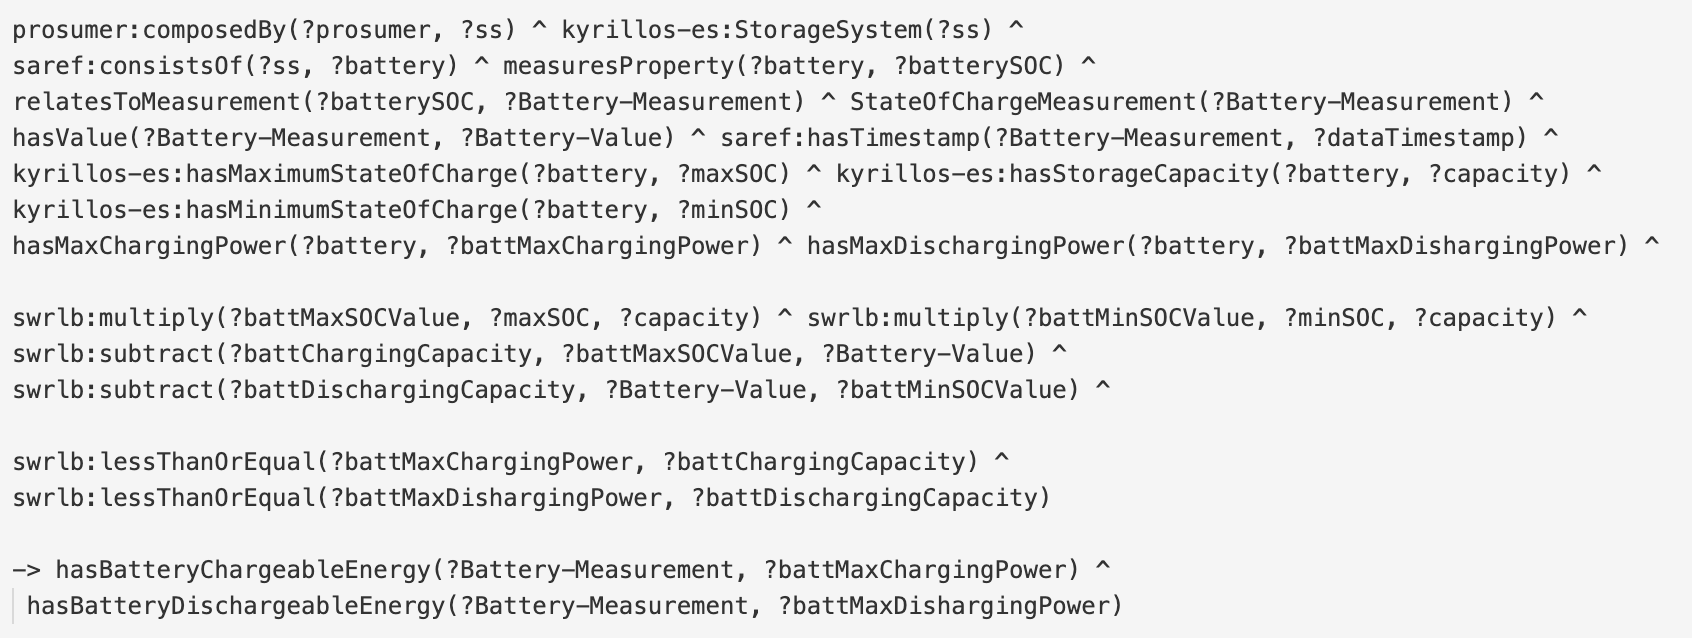
\includegraphics[width=15cm]{images/both <=.png}
    \caption{Screenshot della prima regola.}
    \label{fig:bothlessorequal}
\end{figure}


\subsection{Energia potenzialmente assorbibile = potenza massima di carica e Energia potenzialmente fornibile = capacità di scarica}
[\ref*{fig:charginglessorequal}]  Anche in questo caso la batteria può assorbire al massimo la potenza massima di carica siccome è inferiore o uguale alla capacità di carica,
e invece può fornire al più la capacità di scarica, perchè la potenza di scarica risulta maggiore della capacità.


\begin{figure}[H]
    \centering
    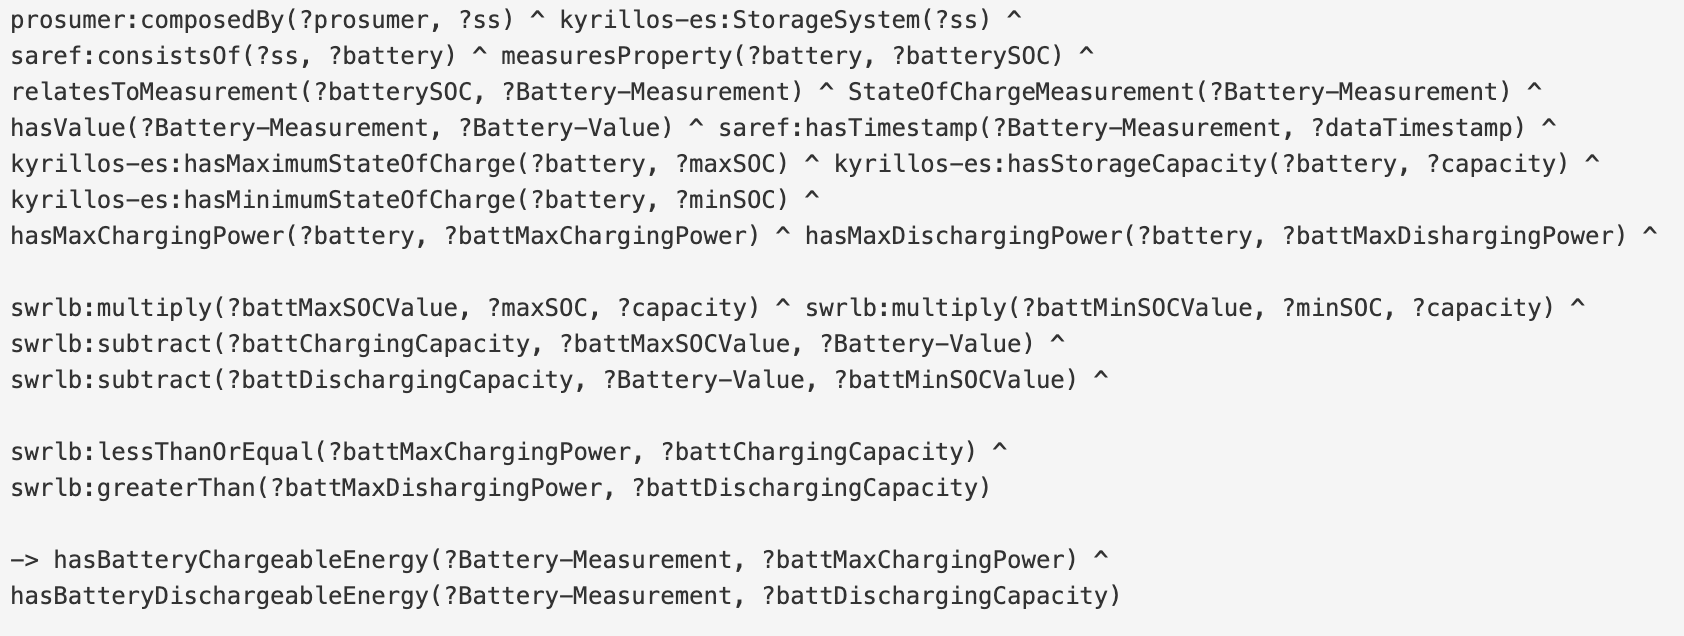
\includegraphics[width=15cm]{images/charging <=.png}
    \caption{Screenshot della seconda regola.}
    \label{fig:charginglessorequal}
\end{figure}


\subsection{Energia potenzialmente assorbibile = capacità di carica e Energia potenzialmente fornibile = potenza massima di scarica}

[\ref*{fig:charginggreater}] In questo caso invece, la capacità di carica è inferiore alla potenza massima, dunque la batteria può assorbibile al massimo la capacità di carica,
mentre può fornire al più la potenza massima di scarica, perchè inferiore o uguale alla capacità di scarica.

\begin{figure}[H]
    \centering
    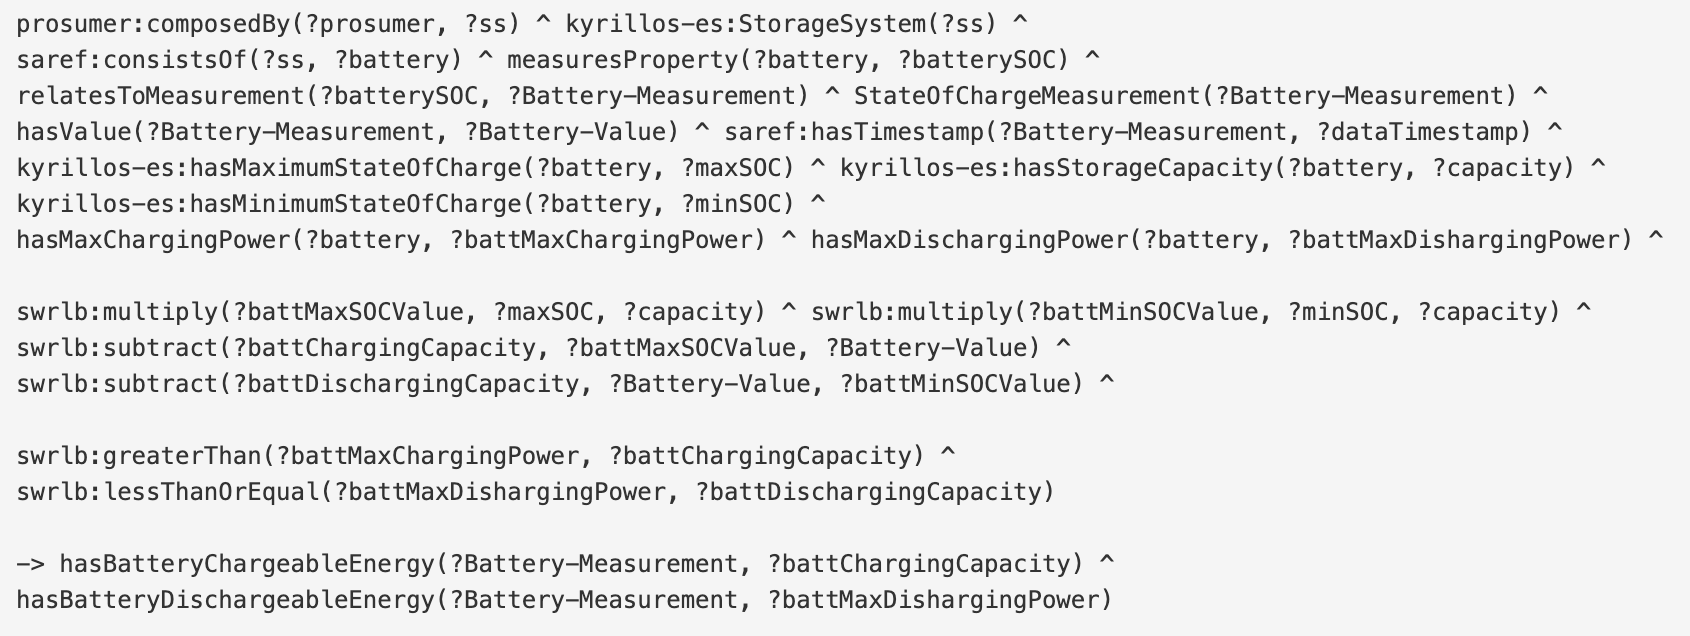
\includegraphics[width=15cm]{images/charging >.png}
    \caption{Screenshot della terza regola.}
    \label{fig:charginggreater}
\end{figure}

\subsection{Energia potenzialmente assorbibile = capacità di carica e Energia potenzialmente fornibile = capacità di scarica}

[\ref*{fig:bothgreater}] Infine c'è il caso in cui la potenza massima sia di carica che di scarica, siano superiori alle rispettive capacità che diventano dunque i valori massimi assorbibili o fornibili dalla batteria.

\begin{figure}[H]
    \centering
    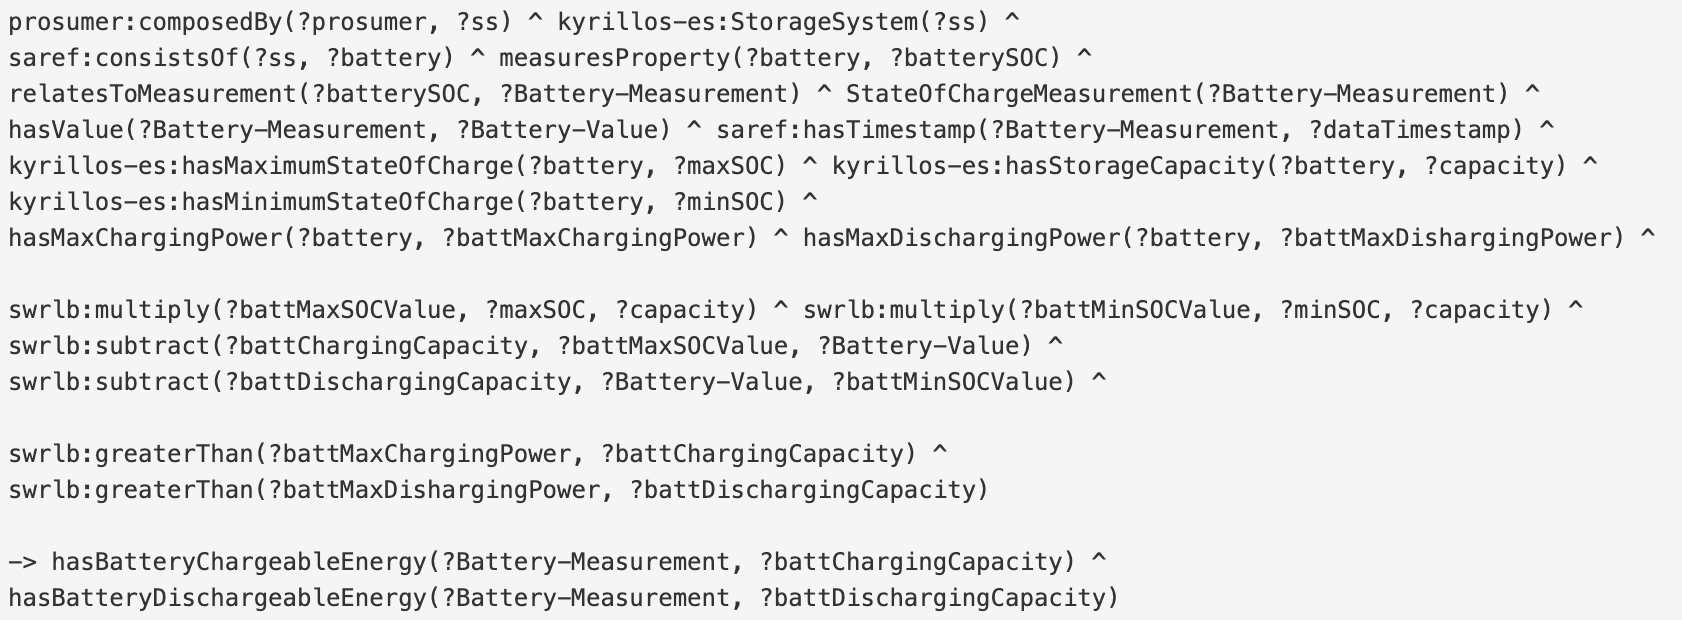
\includegraphics[width=15cm]{images/both >.png}
    \caption{Screenshot della quarta regola.}
    \label{fig:bothgreater}
\end{figure}

\section{SPARQL}\label{sec:sparql}
Nella seguente sezione verranno mostrate le query SPARQL e relativi risultati applicati agli individui creati nell'ontologia.

Si nota che per praticità, in quanto query molto lunghe, verranno mostrate solamente parti delle query come screenshot e i risultati, mentre le query complete sono disponibili nei relativi file di testo che verranno mostrati.


\subsection{PREFIX}
Per leggibilità i prefissi utilizzati per le query SPARQL verranno visionati solamente in questa sezione, siccome ripetitivi per ogni query.

Si può quindi notare l'utilizzo in particolare dell'ontologia \textit{battery}, la nuova ontologia \textit{prosumer}, con anche \textit{SAREF} e \textit{Interconnect}.

\begin{figure}[H]
    \centering
    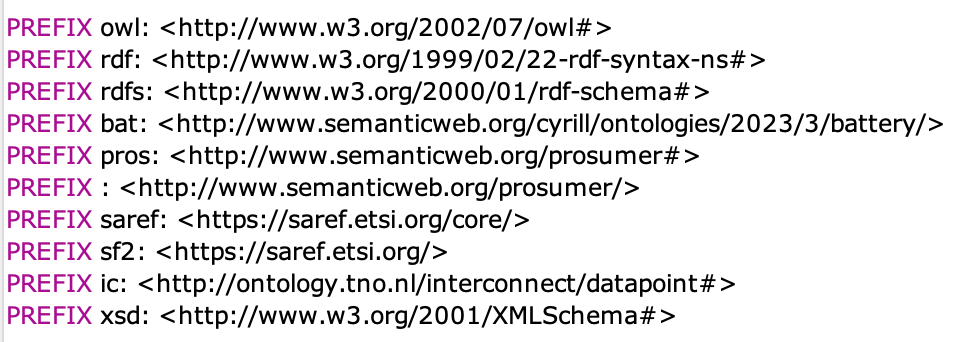
\includegraphics[width=15cm]{images/prefissi.png}
    \caption{Prefissi da anteporre alle query sull'ontologia.}
    \label{fig:prefix}
\end{figure}

\subsection{Query che calcola l'energia che può fornire o assorbire uno Storage System} \label{subquery}

Dato uno Storage System composto da una o più batterie, si vuole calcolare l'energia che il sistema nel suo complesso può assorbire o fornire.

Questa query in pratica utilizza i valori di energia precedentemente calcolati con le regole SWRL, e raggruppa per ogni intervallo di tempo quelli di tutte le batterie presenti nello Storage System del prosumer, in modo da ottenere l'energia che l'intero Storage System può assorbire o fornire.

\begin{figure}[H]
    \centering
    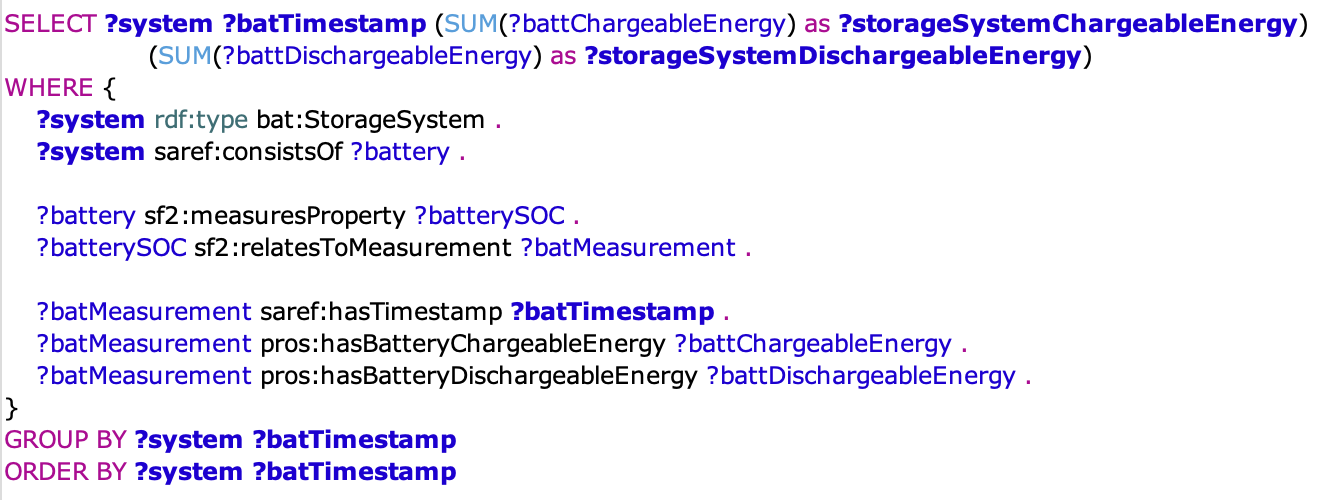
\includegraphics[width=15cm]{images/subquery.png}
    \caption{Query per il calcolo dell'energia che uno Storage System può assorbire o fornire.}
    \label{fig:subquery}
\end{figure}

La query è disponibile nella repository di \href{https://github.com/19eddie/SemanticWeb-Assignment02-03}{Github} nel file \href{https://github.com/19eddie/SemanticWeb-Assignment02-03/blob/main/SPARQL%20energia%20che%20pu%C3%B2%20assorbire%20o%20fornire%20uno%20StorageSystem.txt}{\textit{SPARQL energia che può assorbire o fornire uno StorageSystem.txt}}

Dall'esecuzione della query otteniamo dunque la quantità di energia che ogni Storage System può assorbire e immettere nel relativo timestamp. \ref{fig:subquery_res}

\begin{figure}[H]
    \centering
    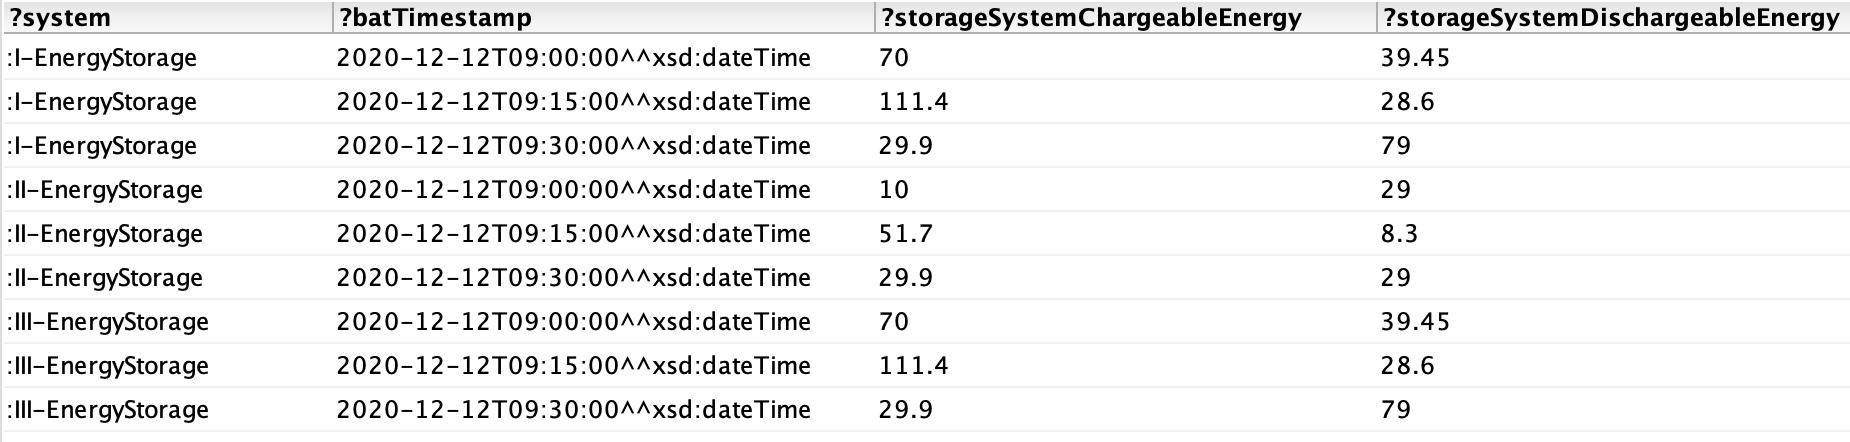
\includegraphics[width=15cm]{images/subquery_res.png}
    \caption{Risultati della query per il calcolo dell'energia che uno Storage System può assorbire o fornire.}
    \label{fig:subquery_res}
\end{figure}

\subsection{Query sul calcolo della flessibilità del contatore M1}

Con flessibilità di M1 si intende indicare il valore minimo e il valore massimo che il contatore può assumere in un determinato intervallo di tempo.
Il valore dipende nello specifico dalle caratteristiche del sistema di accumulo, dal carico richiesto e dalla quantità di energia prodotta dal generatore.
\begin{itemize}
    \item \texttt{M1 minimo:} la batteria viene caricata prelevando energia anche dalla rete;
    \item \texttt{M1 massimo:} la batteria non viene caricata e se il carico è maggiore della produzione, la batteria fornisce energia al carico.
\end{itemize}

\begin{figure}[H]
    \centering
    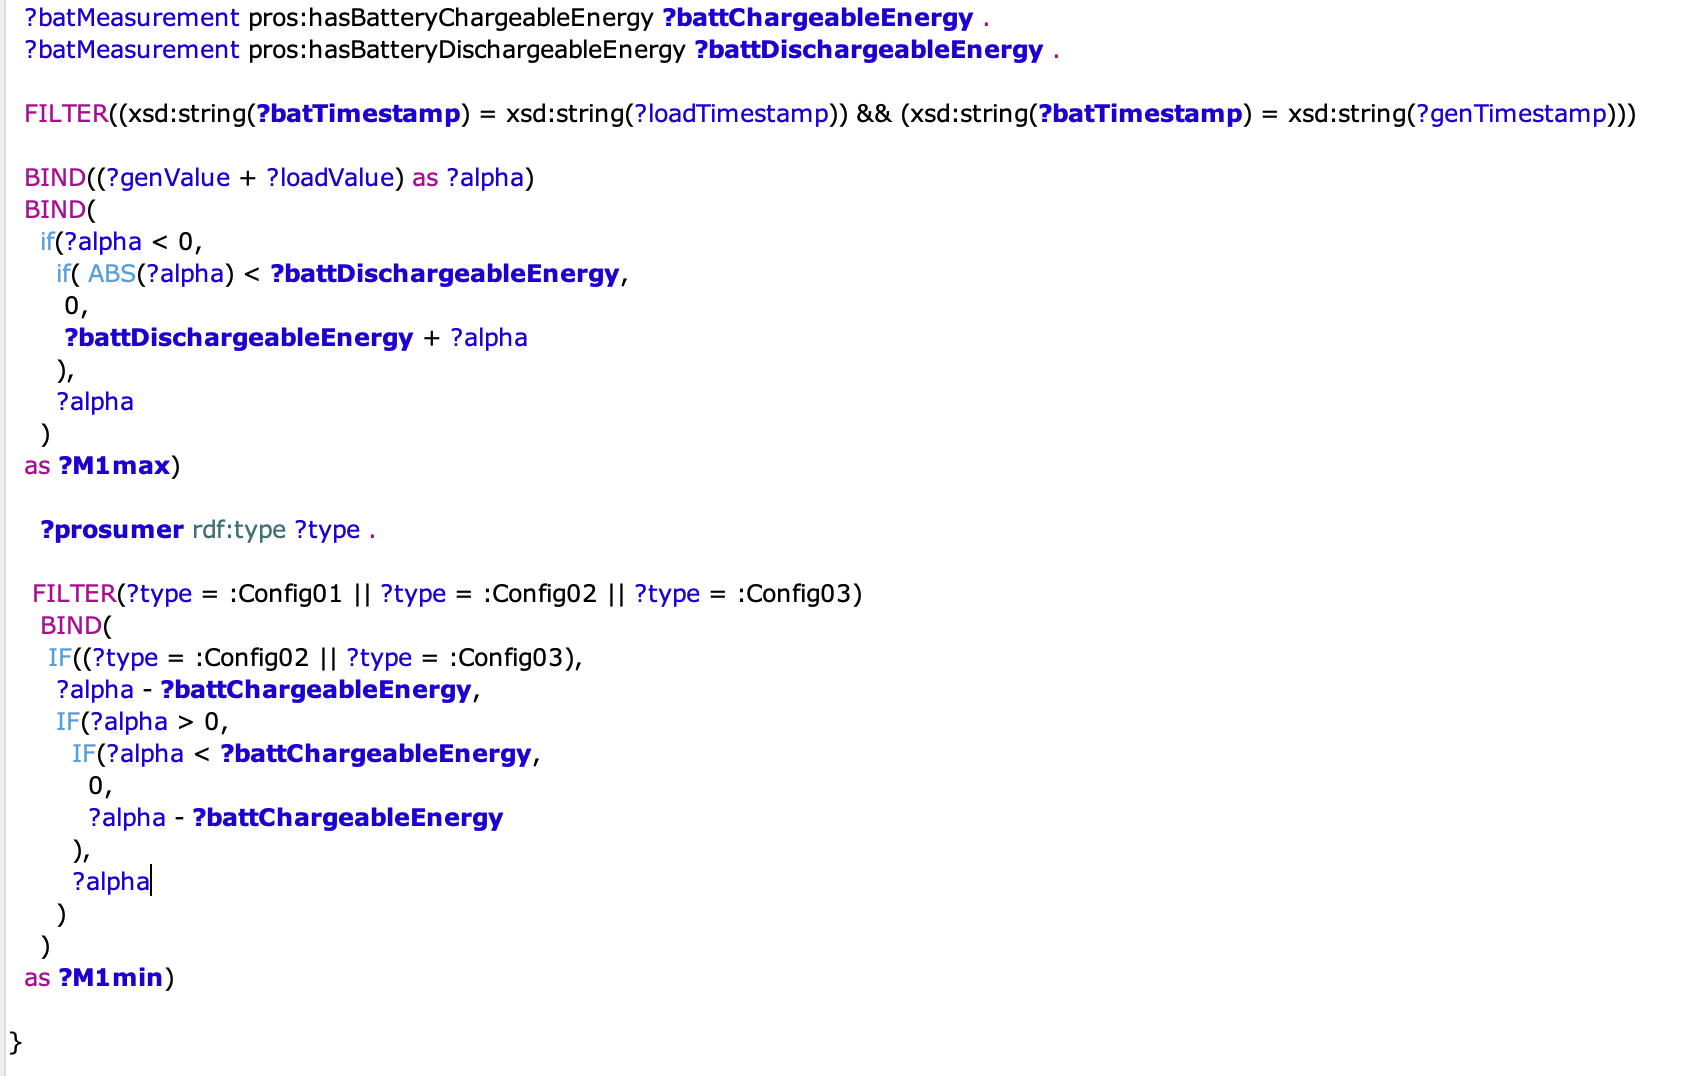
\includegraphics[width=15cm]{images/query_flessibilita.png}
    \caption{Query per il calcolo della flessibilità del contatore M1.}
    \label{fig:query_flessibilita}
\end{figure}

La query utilizza i valori di energia potenzialmente assorbibile o fornibile calcolati con le regole SWRL precedentemente descritte.
Si vuole notare che la query per come è presentata nel file \href{https://github.com/19eddie/SemanticWeb-Assignment02-03/blob/main/SPARQL%20flessibilit%C3%A0.txt}{SPARQL flessibilità.txt} 
purtroppo calcola la flessibilità di ogni batteria, e non di ogni Storage System.
Ciò è dovuto al software che è stato utilizzato per l'implementazione dell'ontologia e l'esecuzione delle query, ovvero Protègè,
che non supporta le subquery nel linguaggio SPARQL \cite{issueprotege}.
Nel caso in cui invece si utilizzasse un software che supporta le subquery, si potrebbe calcolare la flessibilità di ogni Storage System semplicemente inserendo la query \ref{subquery} come subquery e utilizzando quindi \textit{storageSystemChargeableEnergy} e \textit{storageSystemDischargeableEnergy} al posto di \textit{batChargeableEnergy} e \textit{batDischargeableEnergy}.
Ciò vale anche per le query successive.

\begin{figure}[H]
    \centering
    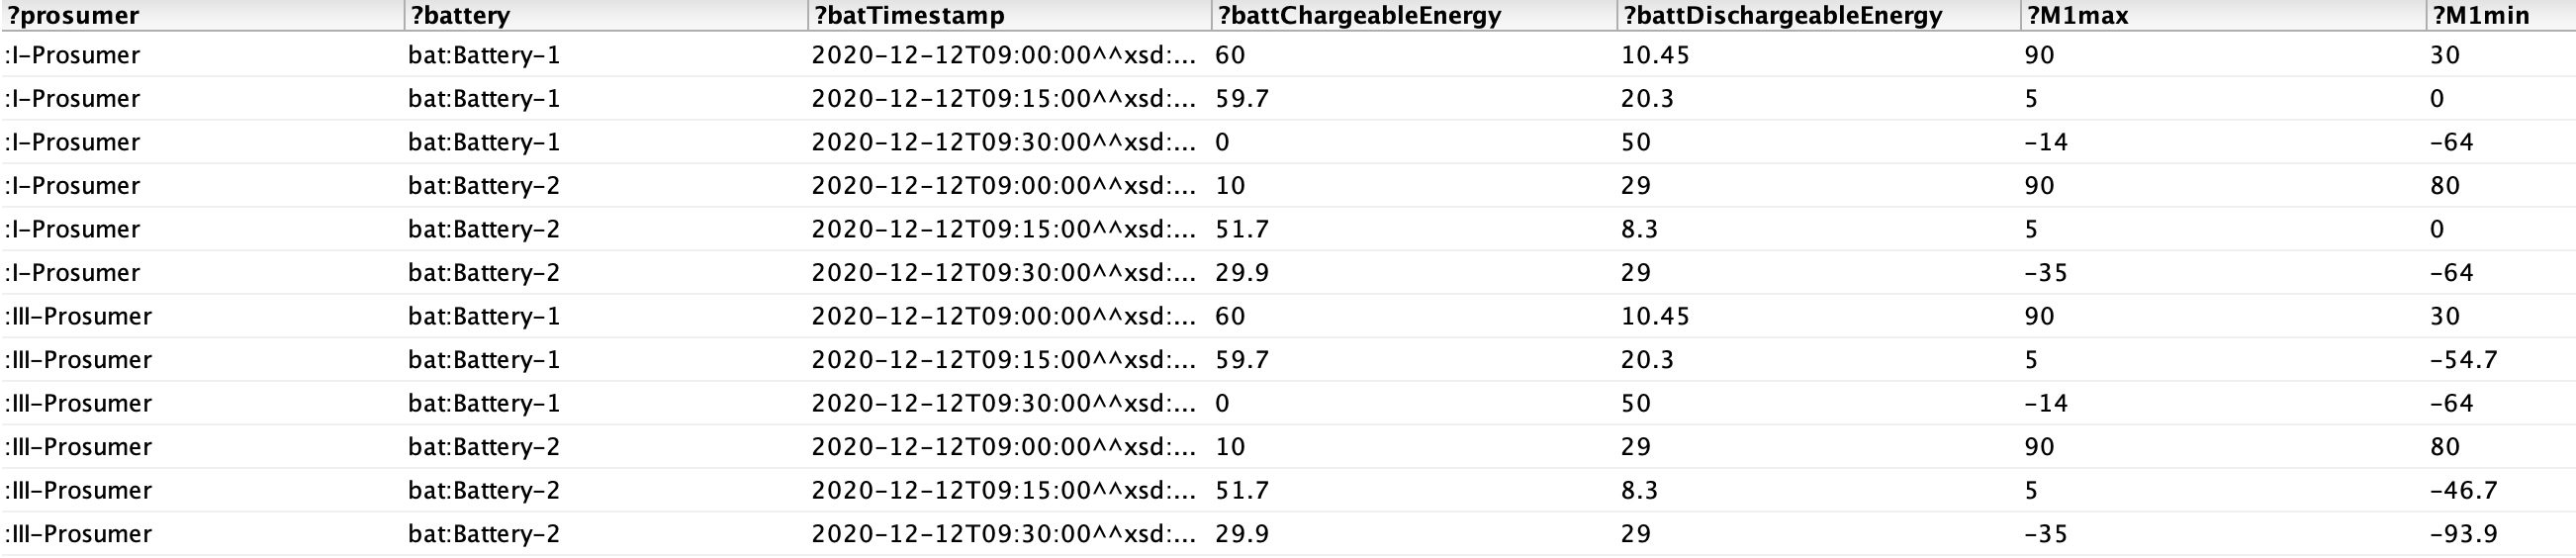
\includegraphics[width=15cm]{images/query_flessibilita_res.png}
    \caption{Risultati della query per il calcolo della flessibilità del contatore M1.}
    \label{fig:query_flessibilita_res}
\end{figure}

Si nota che se il valore di M1 è negativo, indica che l'energia è assorbita dalla rete; se è positivo, indica che l'energia è immessa nella rete.

\subsection{Query per il calcolo di M1 e M2 in prosumer di configurazione 1 e 2}

Le premesse sono le precedenti della query per il calcolo della flessibilità.

Questa query è inerente a prosumer di configurazione 1 e 2, ovvero prosumer che non presentano il contatore M3, in quanto i calcoli sono diversi come sarà mostrato in seguito.

Per entrambe le configurazioni, l'obiettivo è determinare come il sistema di accumulo (batteria) può essere utilizzato per fornire o assorbire energia
in base al carico equivalente e alla produzione di energia del generatore.

\begin{figure}[H]
    \centering
    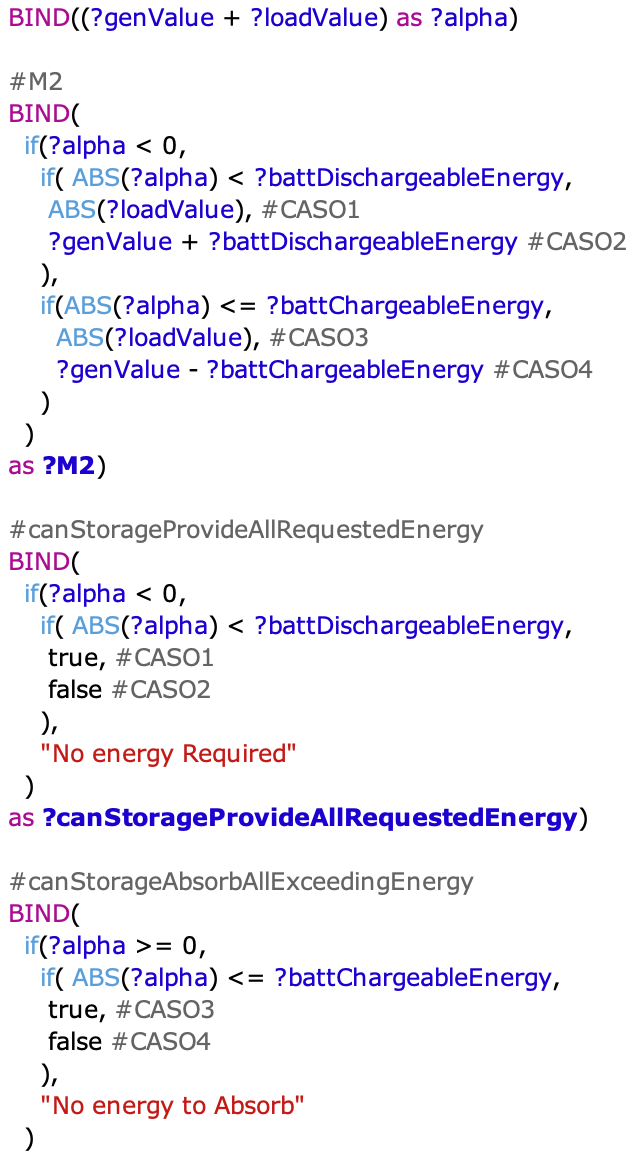
\includegraphics[width=6cm]{images/query_m1m2_config0102.png}
    \caption{Query per il calcolo di M1 e M2 in prosumer di configurazione 1 e 2.}
    \label{fig:query_m1_m2}
\end{figure}

Il calcolo di M2 dipende dal valore di alpha, la differenza tra la generazione di energia e il consumo.

Se alpha è negativo, viene richiesta energia dalla batteria. Se la batteria ha abbastanza energia da fornire, viene soddisfatta tutta la richiesta; altrimenti, viene prelevata il massimo possibile dall'energia del generatore e dalla batteria.
Se alpha è positivo, il prosumer produce più energia di quella richiesta. Se la batteria ha abbastanza capacità di carica, viene utilizzata per assorbire tutta l'energia in eccesso; altrimenti, la batteria viene caricata con il massimo possibile.
Nel calcolo di M1, il valore rappresenta l'energia totale scambiata con la rete, includendo l'energia del generatore, l'energia prelevata e fornita dalla batteria e l'energia assorbita o immessa dalla rete.
M1 viene ottenuto sommando il valore di M2 al consumo.

\begin{figure}[H]
    \centering
    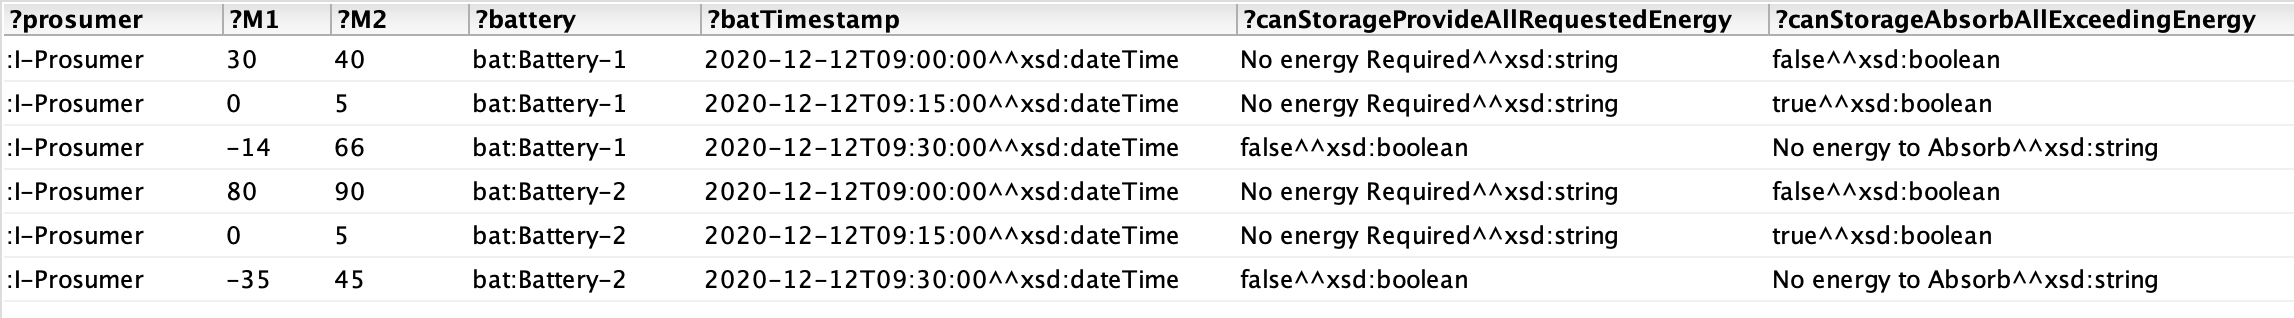
\includegraphics[width=15cm]{images/query_m1m2_config0102_res.png}
    \caption{Risultati della query per il calcolo di M1 e M2 in prosumer di configurazione 1 e 2.}
    \label{fig:query_m1_m2_res}
\end{figure}

La query completa si trova nel file \href{https://github.com/19eddie/SemanticWeb-Assignment02-03/blob/main/SPARQL%20M1%20e%20M2%20in%20config01%20e%20config02.txt}{\textit{SPARQL M1 e M2 in config01 e config02.txt}}.

\subsection{Query per il calcolo di M1, M2 e M3 in prosumer di configurazione 3}

Infine si vuole calcolare M1, M2 e M3 per prosumer di configurazione 3.

M2 rappresenta l'energia prodotta dal generatore, mentre M3 rappresenta l'energia scambiata con la batteria ed è determinata dalla differenza tra l'energia prodotta dal generatore e l'energia assorbita dal carico del prosumer.
Se il prosumer richiede energia dalla batteria, M3 assume il valore dell'energia richiesta, a meno che la batteria non abbia abbastanza energia disponibile, in tal caso assume il massimo di energia scaricabile dalla batteria. Se il prosumer produce più energia di quella richiesta,
M3 assume il valore dell'energia in eccesso che può essere assorbita dalla batteria, a condizione che abbia abbastanza capacità di carica; altrimenti, assume il massimo valore di capacità di carica della batteria, ma negativo.
Infine, M1 rappresenta il totale di energia scambiata con la rete, includendo l'energia prodotta dal generatore, l'energia scambiata con la batteria e il valore del carico del prosumer.

\begin{figure}[H]
    \centering
    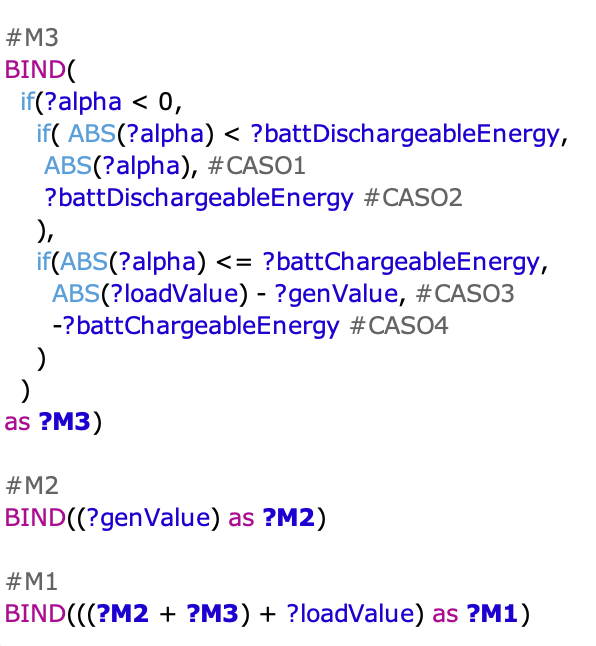
\includegraphics[width=7cm]{images/query_m3.png}
    \caption{Query per il calcolo di M1, M2 e M3 in prosumer di configurazione 3.}
    \label{fig:query_m3}
\end{figure}

La query completa si trova nel file \href{https://github.com/19eddie/SemanticWeb-Assignment02-03/blob/main/SPARQL%20M1%2C%20M2%2C%20M3%20in%20config03.txt}{\textit{SPARQL M1, M2, M3 in config03.txt}}.


\begin{figure}[H]
    \centering
    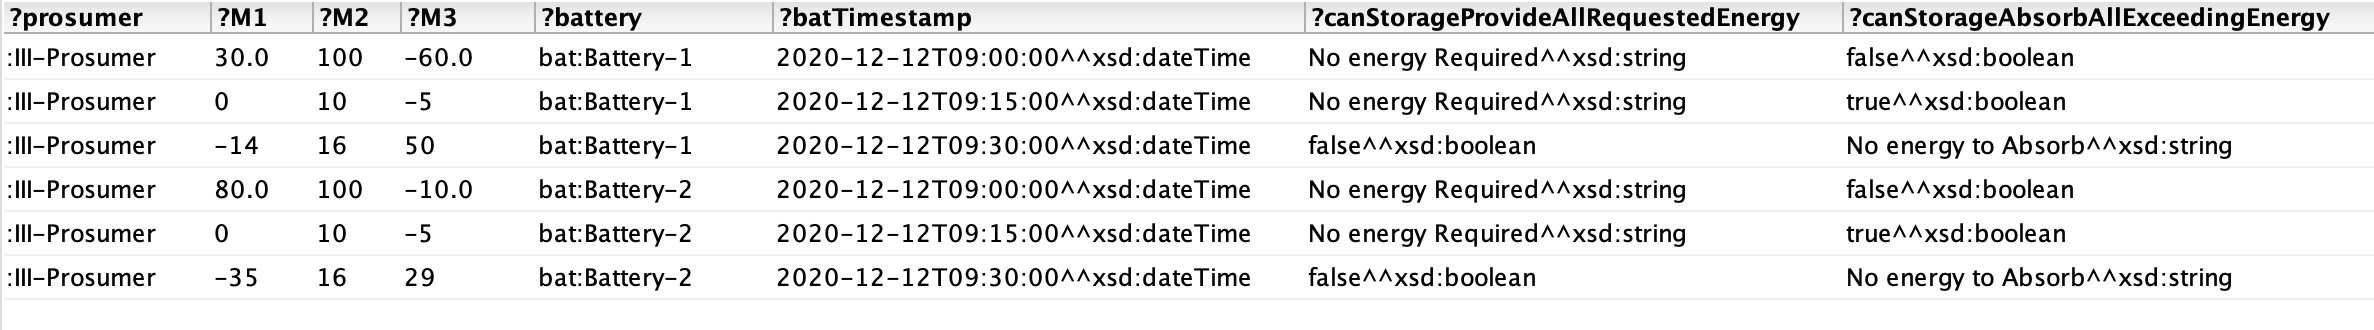
\includegraphics[width=15cm]{images/query_m3_res.png}
    \caption{Risultati della query per il calcolo di M1, M2 e M3 in prosumer di configurazione 3.}
    \label{fig:query_m3_res}
\end{figure}
\chapter{Conclusioni}

\bibliographystyle{plain}
\bibliography{bibliography}

\end{document}